% Chapter Template

\chapter{Implementation Prototype} % Main chapter title

\label{Chapter5} % Change X to a consecutive number; for referencing this chapter elsewhere, use \ref{ChapterX}

\lhead{Chapter 5. \emph{Implementation Prototype}} 
% Introduction for implementation
In this chapter we have developed a prototype for the scheme proposed in section \ref{propopsedsol}. We have chosen as an implementation platform the Android Nexus 5 smart phone. The device offers enough sensors to perform biometric and behavioural analysis \footnote{The full range of sensors supported by the Android platform can be found here: http://developer.android.com/guide/topics/sensors/sensors\_overview.html (accessed on 28.05.2014)}. These resources will be used to demonstrate that the scheme can be implemented using similar dedicated hardware that may offer more security features.

We have included a brief overview of the Android development model and the platform's security features in appendix \ref{AppendixB}. This information provides an introduction for understanding the principles used in the implementation of the prototype.

\section{Implementation overview}
\label{impleoverview}
% Introduction with UAService
The Android token unlocking scheme is designed to work as a bound service. It is implemented in the ``UAService'' \footnote{The name of the class stands for User Authentication Service} class. Feedback is provided to clients either after an explicit request or through periodic broadcasts.

% Mention independent services for each mechanism and why
Each authentication mechanism that participates in the scheme may have different requirements for sampling and processing data. As an example, voice recognition can gather optimal data during a phone call \footnote{Call events can be intercepted by registering a listener for the PHONE\_STATE event}, while face recognition when the phone screen is unlocked. Therefore, to enable more flexibility in the individual mechanisms' implementation, they are developed as independent services.

% Management of authentication mechanisms
``UAService'' communicates with the authentication mechanisms by binding to their service. On predefined time intervals it requests the confidence level and weight of each mechanism. Using this data it then calculates the overall result according to the design in section \ref{authfeedback}. Feedback is sent back to each registered client for interpretation.

\section{Implementation details}
% Introduction (can expand)
This section presents the implementation of the design proposed in section \ref{propopsedsol}. The full source code for the prototype can be downloaded from github \footnote{https://github.com/cristiantoader/fyp-pico}. 

The structure of the Android application is presented in figure \ref{fig:overview}. Each colour represents an Android component (e.g. activity, service). This should provide a better understanding of the overall design. A full detailed UML diagram could not be included with this dissertation, but can be downloaded from github \footnote{https://github.com/cristiantoader/fyp-pico/blob/master/PicoUserAuthenticator/dissertation/Pictures/detailed-uml.png}.
\begin{figure}[h]
    \centering
    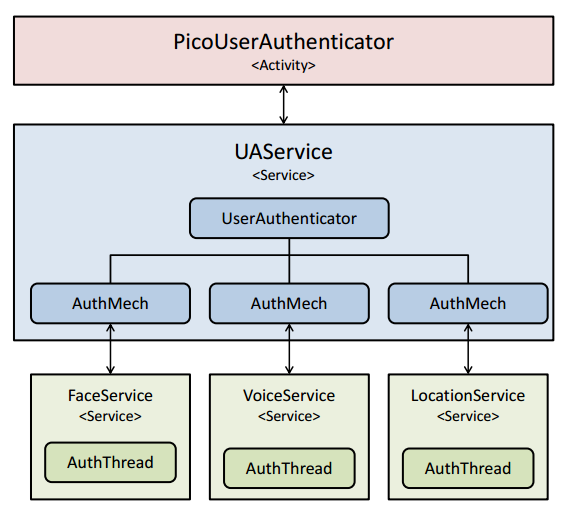
\includegraphics[width=0.7\textwidth]{Pictures/overview-uml}
    \caption{Authenticator design overview}
    \label{fig:overview}
\end{figure}

\subsection{UAService}
% UAService
The token unlocking mechanism is started using the ``PicoMainActivity'' class, which acts as a Pico client. The scheme itself is developed to be used by binding the ``UAService'' component. An UML diagram of the different components related to ``UAService'' is attached in figure \ref{fig:uaservice}.
\begin{figure}[h]
    \centering
    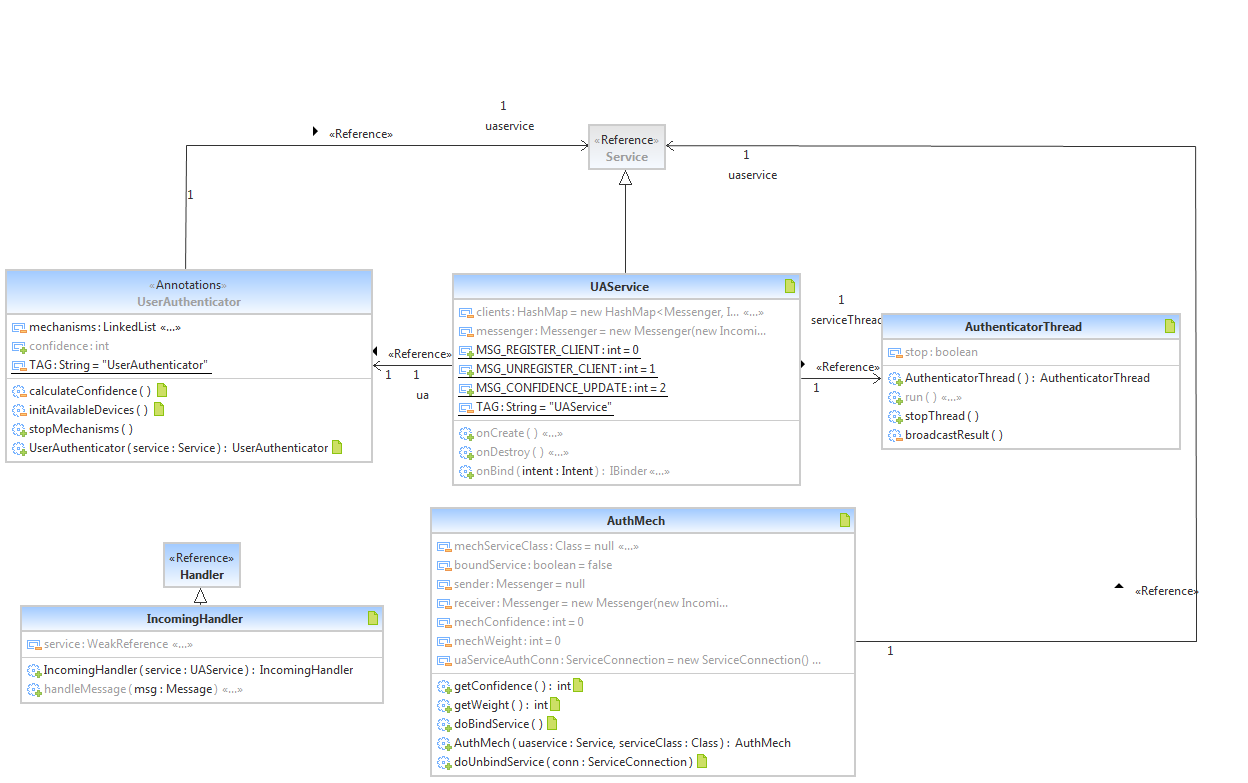
\includegraphics[width=\textwidth]{Pictures/uaservice}
    \caption{UAService components}
    \label{fig:uaservice}
\end{figure}

% UAService and lifetime
``PicoMainActivity'' starts ``UAService'' using the ``Context.startService()'' method. Communication is enabled by binding to ``UAService'' using ``Context.bindService()''. This approach protects the lifetime of the authenticator. When ``PicoMainActivity'' gets sent to background and loses control of the screen, ``UAService'' is not explicitly unbound. This guarantees that the service will continue running in the background, and should also prevent malicious components from stopping it. 

% UAService, central node.
Clients need to bind ``UAService'' to receive authentication updates. When bound, communication is enabled by exchanging ``Messenger'' objects using the IBinder interface. A ``Messenger'' allows another component to send ``Message'' objects, and defines how they are handled by the receiver through an ``IncomingHandler''. The ``Messenger'' queues all requests on a single thread, and therefore the application does not require to be thread safe. 

When bound by a client, the ``IncomingHandler'' used by ``UAService''  exposes the following API defined by the ``what'' parameter of a received ``Message'': 
\begin{description}
  \item[MSG\_REGISTER\_CLIENT] \hfill \\
  Used for registering a client for periodic broadcasts of the current authentication confidence level. Feedback is provided at a fixed time interval of 1000ms \footnote{An alternative implementation explored in the project was to have each client also register a confidence level using the ``arg1'' parameter of a ``Message''. In this case, the authenticator would only provide each client with a locked/unlocked result. However, this would shift the meaning of client to that of an authentication session, with state managed by the unlocking scheme. A client would therefore have multiple connections, requiring more ICC. Since all ``Messenger'' requests made to ``UAService'' are queued to a single thread, this would slow down the feedback process and possibly lead to a denial of service attack. Therefore we have chosen to reduce the communication overhead, and have each client manage the status of its authentication sessions based on the confidence level provided by the unlocking scheme.}.

  \item[MSG\_UNREGISTER\_CLIENT] \hfill \\
  Used for any application component to unregister as a listener from ``UAService''.
  
  \item[MSG\_GET\_STATUS] \hfill \\
  Used by a client for requesting an explicit authentication status update.
\end{description}

% Communication with authentication mechanisms
The ``UAService'' service wraps an ``UserAuthenticator'' proxy object that implements most of its functionality. The ``UserAuthenticator'' is responsible for collecting data from authentication services, and computing the final confidence level. The fact that the mechanisms are independent services is hidden from the ``UserAuthenticator'' using ``AuthMech'' observer objects. Each ``AuthMech'' starts and binds an authentication mechanism, listens for confidence level updates, and keeps track of the most recent value.
 
% Authentication mechanism side
Each authentication mechanism service extends the ``AuthMechService'' abstract class. This defines them as bound services with the same ``IncomingHandler'' implementation. The communication with ``AuthMech'' is therefore standardized, providing the following ``Messenger'' API:
\begin{description}
  \item[AUTH\_MECH\_REGISTER] \hfill \\
  Used for registering the ``UAService'' client to the ``AuthMechService''.
  
  \item[AUTH\_MECH\_UNREGISTER] \hfill \\
  Used for unregistering the ``UAService'' client from the ``AuthMechService''.
\end{description}    

% TODO: calculate the final result.  
  
\subsection{Authentication mechanisms}
\label{implauthmech}
% Introduction for authentication mechanisms
In order to create a functional prototype, we have implemented a number user authentication mechanisms. The result quality of each mechanisms is outside the scope of this project. Their sole purpose is to demonstrate that sensor data offered by smart phones can be used to implement biometric and behavioural analysis.

% Mechanism requirements 
When developing an individual authentication mechanism, the following abstract requirements need to be satisfied: 
\begin{enumerate}
	\item The result needs to be quantifiable in the form of a percentage ranging from 0 to 100, where 100 means that the mechanism has $100\%$ confidence that the owner of the token is present.
	\item The mechanism needs to support continuous authentication.
	\item The authentication process needs to be effortless and preferably unobtrusive for the user.
\end{enumerate}
A list of authentication mechanism examples that can be implemented on the Android platform is presented in appendix \ref{AppendixC}.

% AuthMechService functionality
Each mechanism developed for this scheme extends the ``AuthMechService'' abstract class. As mentioned, this class defines the mechanism as a bound service. The communication with ``UAService'' is standardized by implementing ``Service.onBind()'' to register the same ``IncomingHandler'' implementation. Furthermore, ``AuthMechService'' defines the decay implementation of a mechanism's weight. This is developed using a ``Handler'' object that schedules a ``Runnable'' to execute at a predefined time interval. The ``Runnable'' is responsible for decreasing the mechanism's weight and sending the result to the corresponding ``AuthMech''. Figure \ref{fig:authmechservice} provides an overview of the components interacting with ``AuthMechService''.
\begin{figure}[h]
    \centering
    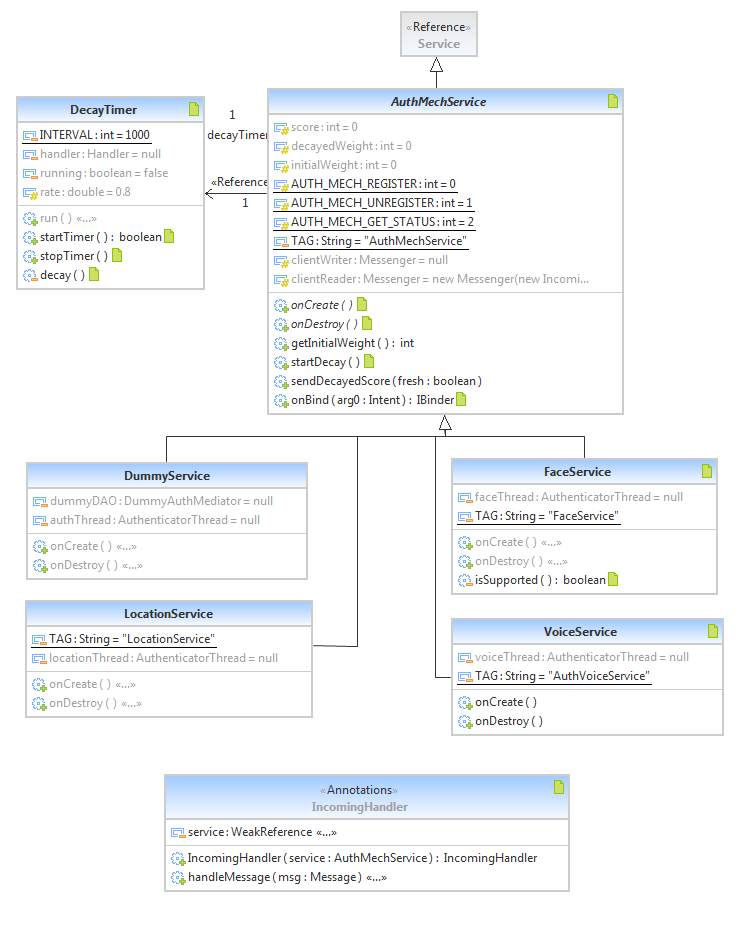
\includegraphics[width=\textwidth]{Pictures/authmechservice}
    \caption{AuthMechService components overview.}
    \label{fig:authmechservice}
\end{figure}

% General application design
Although it is not enforced, each authentication mechanism has the same general design. The mechanism's ``Service.onCreate()'' method initialises the weight of the mechanism, and starts a thread responsible for periodically collecting sensor data using an access object (DAO). The samples are analysed using a class that mediates interaction with other components and libraries. After each successful analysis, the result is sent back to the corresponding ``AuthMech'' and the decay process is started using ``AuthMechService.startDecay()''.

% Euclidean distance conversion
The biometric libraries used in the prototype provide feedback as an Euclidean distance. To convert it to a percentage confidence level, we define for each mechanism an acceptable threshold. Any result above the threshold is considered too high and is truncated to its value. Using equation \ref{eq:euclideantoprob} we convert the Euclidean distance to a confidence level. Dividing the distance over the threshold yields a value between 0 and 1, where 1 is a very large distance and hence a bad result. By using one minus this value we invert the meaning. Values will range between 0 and 1, and 1 corresponds to a confidence level of $100\%$. This result is $P(E|H)$ from equation \ref{eq:final}.

\begin{equation} 
\label{eq:euclideantoprob}
P(E|H) = 1 - \frac{distance}{THRESHOLD}
\end{equation}

% Do Bayesian update
Having known $P(E|H)$ we continue to calculate $P(H|E)$ by using the Bayesian update formula defined in equation \ref{eq:final}. When calculating the final value of the mechanism, we multiply $P(H|E)$ with the current decayed weight.

% Listing mechanisms with promises of future details
The following mechanisms have been implemented as part of the prototype: voice recognition, face recognition, location analysis, and a dummy mechanism used for testing. The next sections will provide details regarding their functionality and implementation process.

\subsubsection{Dummy mechanism}
% Introduction: what it does, why it was developed
A dummy authentication mechanism was developed for testing the overall scheme. It produces random confidence levels within a predefined range, which provides a controlled testing environment. An overview of the components involved in the dummy mechanism are shown in figure \ref{fig:dummy}
\begin{figure}[h]
    \centering
    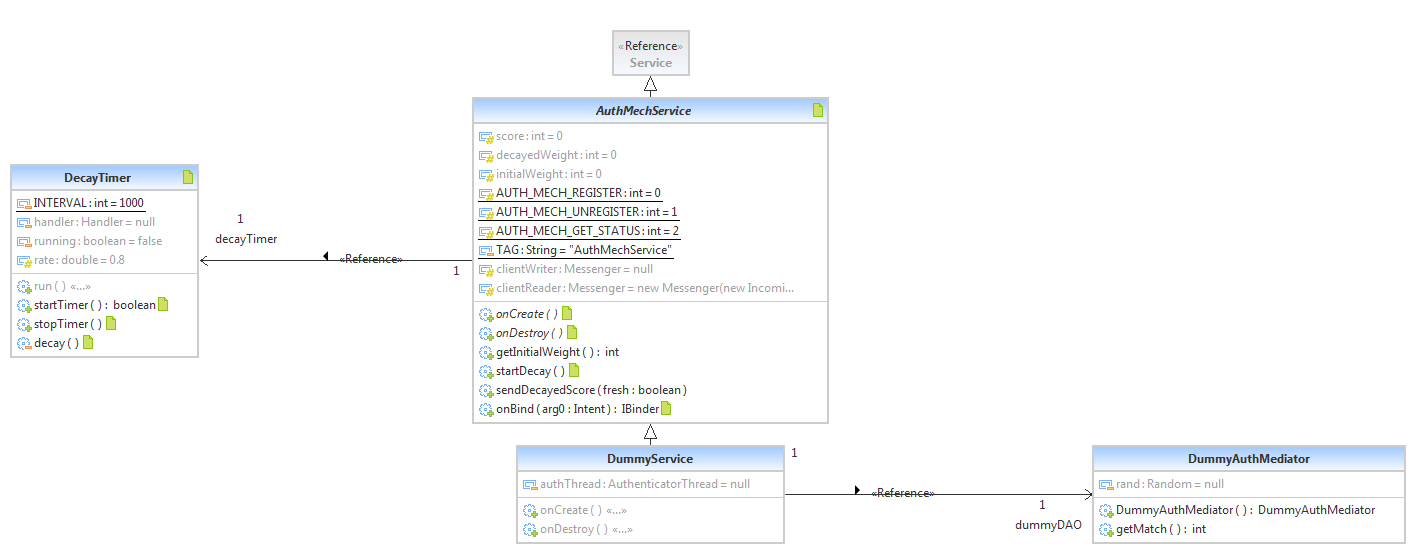
\includegraphics[width=\textwidth]{Pictures/dummy}
    \caption{Dummy mechanism}
    \label{fig:dummy}
\end{figure}

% General implementation detail
The mechanism was developed in the ``DummyService'' class and was designed consistently with the application model. Its ``DummyService.onCreate()'' method creates an authentication thread that periodically generates random values and sends them to ``UAService''. It does not use any DAO, in order not to over complicate its implementation. The random values are generated using a ``DummyAuthMediator'' object. Once the mechanism's confidence level is calculated, the weight decay process is started using ``AuthMechService.startDecay()'' and result updates are sent back to ``UAService''.

\subsubsection{Voice recognition}
% Introduction to mechanism
The voice recognition mechanism is implemented in the ``VoiceService'' class and extends the ``AuthMechService'' abstract class. The ``VoiceService.onCreate()'' method starts a thread that periodically gathers data from the microphone, performs biometric authentication, and produces a confidence level. An overview of the components involved in this mechanism is presented in figure \ref{fig:voice}.
\begin{figure}[h]
    \centering
    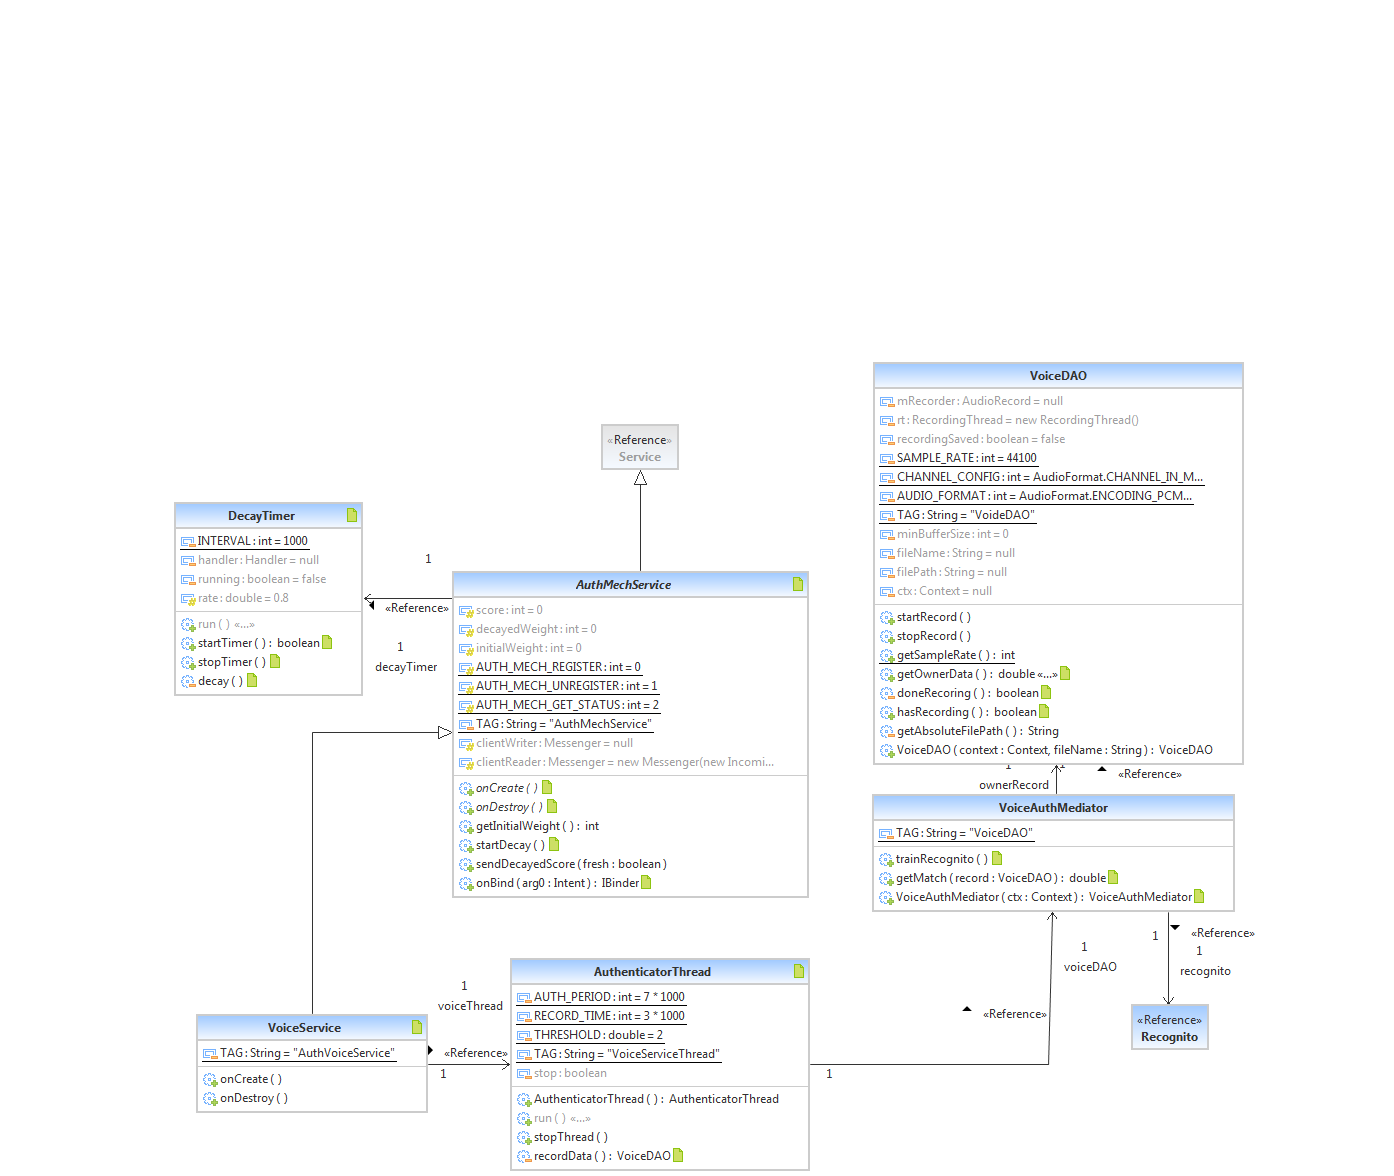
\includegraphics[width=\textwidth]{Pictures/voice}
    \caption{Voice recognition overview.}
    \label{fig:voice}
\end{figure}

% Library used for implementation
The library used for biometric voice recognition is called Recognito \footnote{The library can be downloaded using github from the following link: https://github.com/amaurycrickx/recognito}, and was developed by Amaury Crickx. It uses a text independent speaker recognition algorithm developed in Java (SE). Its author claims very good results in scenarios with minimal background noise \footnote{It was tested by its author on TED talks such as:  https://www.ted.com/talks/browse (visited on 06.01.2014)}.

% Hack to compile with the library
Porting Recognito for Android required no changes. However, in order to package the library, a subset of the ``rt.jar'' Java (SE) library is needed for sound file formats. Including the full ``rt.jar'' is not possible due to a package name collision with Android ``javax.*'' system libraries. Therefore, we have included only the ``javax.sound.*'' package using a custom jar. This was purely done to trick the Android Java compiler to build the application. Using ``javax.sound'' features would generate a runtime error. Therefore, we only use Recognito functions which require direct data input, without any knowledge of sound file formats.

% Recording configuration
In order to gather and manage samples compatible with the Recognito library we have created the ``VoiceDAO'' class. Microphone input is gathered using the following predefined configuration:
\begin{itemize}
	\item Sample rate: 44100
	\item Channel configuration: AudioFormat.CHANNEL\_IN\_MONO
	\item Audio format: AudioFormat.ENCODING\_PCM\_16BIT
\end{itemize}

% More DAO recording stuff.
The minimum buffer size required by ``VoiceDAO'' is device dependant and pre-calculated when data recording is initiated using ``VoiceDAO.startRecord()''. The class wraps an Android ``AudioRecord'' object used for gathering microphone data. When the recording is stopped, data is stored in the object with the option of saving to disk by calling ``VoiceDAO.saveRecording()''. 

% Library Mediator
The ``VoiceAuthMediator'' class was created to mediate calls to the Recognito library. When initialised, it loads the owner configuration, and a predefined set of background noises. It then creates a ``Recognito'' object and trains it using the data. This is performed using the ``Recognito.createVocalPrint()'' method.

% Getting confidence level
Every predefined time interval, the ``VoiceService'' authentication thread records data in ``double[]'' format using a ``VoiceDAO'' object. It uses the ``VoiceAuthMediator'' to analyse the sample. This returns the Euclidean distance to the closest match, which is either the owner, or one of the background noises used for training. We convert the Euclidean distance from ``VoiceAuthMediator'' to a percentage using equation \ref{eq:euclideantoprob}. The final confidence is computed, stored in the service, and the decay process is started. Whenever the weight is modified, a ``Message'' is sent to the corresponding ``AuthMech'' and updates its value. 
 
\subsubsection{Face recognition}
\label{implface}
% Introduction: brief description of the implementation
The face recognition mechanism was implemented in the ``FaceService'' class and extends ``AuthMechService''. When created, the service starts an authentication thread that periodically collects data from the camera, performs biometric face recognition, and produces a confidence level. An overview of the components involved in the face recognition mechanism is shown in figure \ref{fig:face}.
\begin{figure}[h]
    \centering
    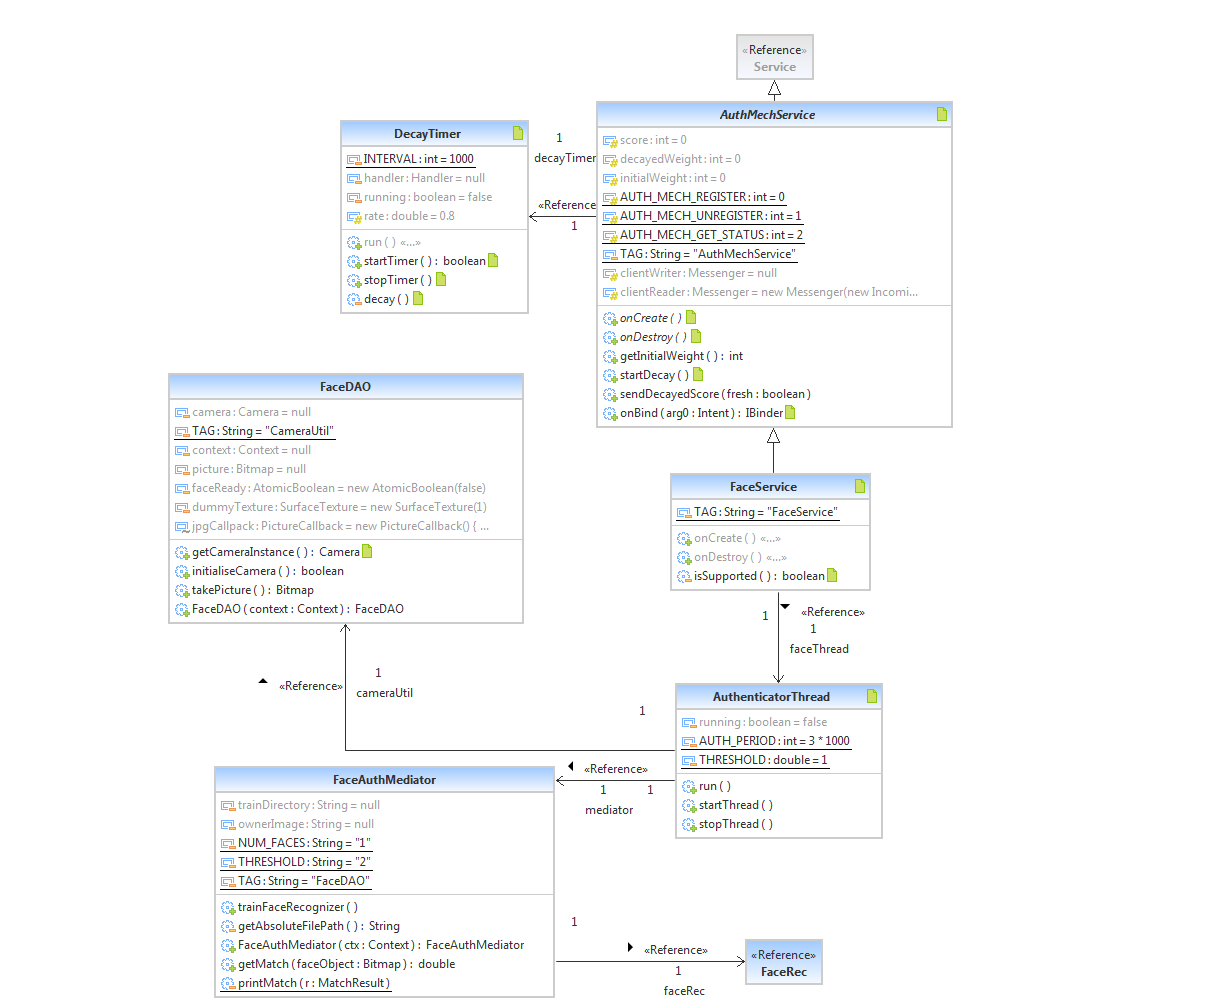
\includegraphics[width=\textwidth]{Pictures/face}
    \caption{Face recognition overview.}
    \label{fig:face}
\end{figure}

% Javafaces library
Face recognition is implemented using a modified version of the ``Javafaces'' library \footnote{The ``JavaFaces'' library is maintained at the following address: https://code.google.com/p/javafaces/}. It is written entirely using Java (SE), but unfortunately uses the ``javax.imageio.'' package that is not available in the Android API. A considerable amount of code needed to be ported for the Android platform. Although not currently optimised for public use, the new library is available at the following link: https://github.com/cristiantoader/JavafacesLib.

% Javafaces changes for porting to Android
We will briefly present the changes made when porting the ``Javafaces'' library. The ``BufferedImage'' class had to be replaced by its closest Android equivalent, which is ``Bitmap''. This required a number of adaptations due to differences between the two classes. For example, ``BufferedImage'' grey-scale images use a single colour channel for the grey intensity value. This had to be changed to the Bitmap format that uses all 3 channels. Additional modifications were required due to data type mismatches, as well as other related issues. Furthermore, The API was modified to support direct ``Bitmap'' input in order to add more flexibility and lighten the main code of the authenticator. 

% Authentication process
Each predefined time interval the ``FaceService'' authentication thread collects a picture from the camera. Its validity is determined using the Android ``FaceDetector'' class. If the image contains a face it continues to be processed, otherwise the weight decays until a new data sample is collected. The image collection and validation was simplified by developing the ``CameraDAO'' class.

The ``FaceAuthMediator'' class was implemented to mediate calls to the ``Javafaces'' library. When the authentication thread is started, a ``FaceAuthMediator'' is created and used for training the biometric recognizer. It then analyses face data sampled from ``CameraDAO'' in order to produce a result. The return value represents the Euclidean distance between the face captured from the camera and the registered owner face. This distance is transformed into a percentage confidence level using equation \ref{eq:euclideantoprob}, and the decay process is restarted.  

% Gather picture with no notification: shutter sound
The Android API does not easily allow for a Camera picture to be taken without any sort of notification to the user. Both a shutter sound and a visual preview display should be present. The sound can be disabled by not providing a shutter callback function when calling the Camera.takePicture() method. 

% Gather picture with no notification: shutter sound
Disabling the user preview of the camera was more difficult to achieve. The solution was to exploit an Android feature that allows to render the preview in a ``SurfaceTexture'' object. This satisfies the API's requirement to have a visual display preview for the camera, while the ``SurfaceTexture'' itself does not need to be displayed on screen. Therefore a picture can be taken from a background service without any interruption to the user.

% Issue of image too large
Another problem encountered by the face recognition service is data sizes. When the ``Javafaces'' library performed face recognition, the device was running out of memory. This caused the app to be closed by the Android OS. To fix this issue, all images collected from the camera are resized to $50\%$ before they are processed.

% Results
The library combined with the Android SDK does not provide accurate results. The reason is that it requires an input image perfectly embedding the face of the user. Unfortunately, although the Android SDK offers face detection, it only provides the location of the midway coordinate, and distance between the eyes. Using this data alone, an accurate crop cannot be made. As a solution, yet another library is needed to properly detect face regions. This would provide better input data and increase the precision of the mechanism.

\subsubsection{Location analysis}
% Introduction: short description of the mechanism
This mechanism is based on gathering location data and using it to generate a probability that the owner is present. This is implemented in the ``LocationService'' class and extends the ``AuthMechService'' abstract class. Data is collected periodically using the ``LocationManager'' provided by the Android API. An overview of the components involved in the location analysis mechanism is shown in figure \ref{fig:location}.
\begin{figure}[h]
    \centering
    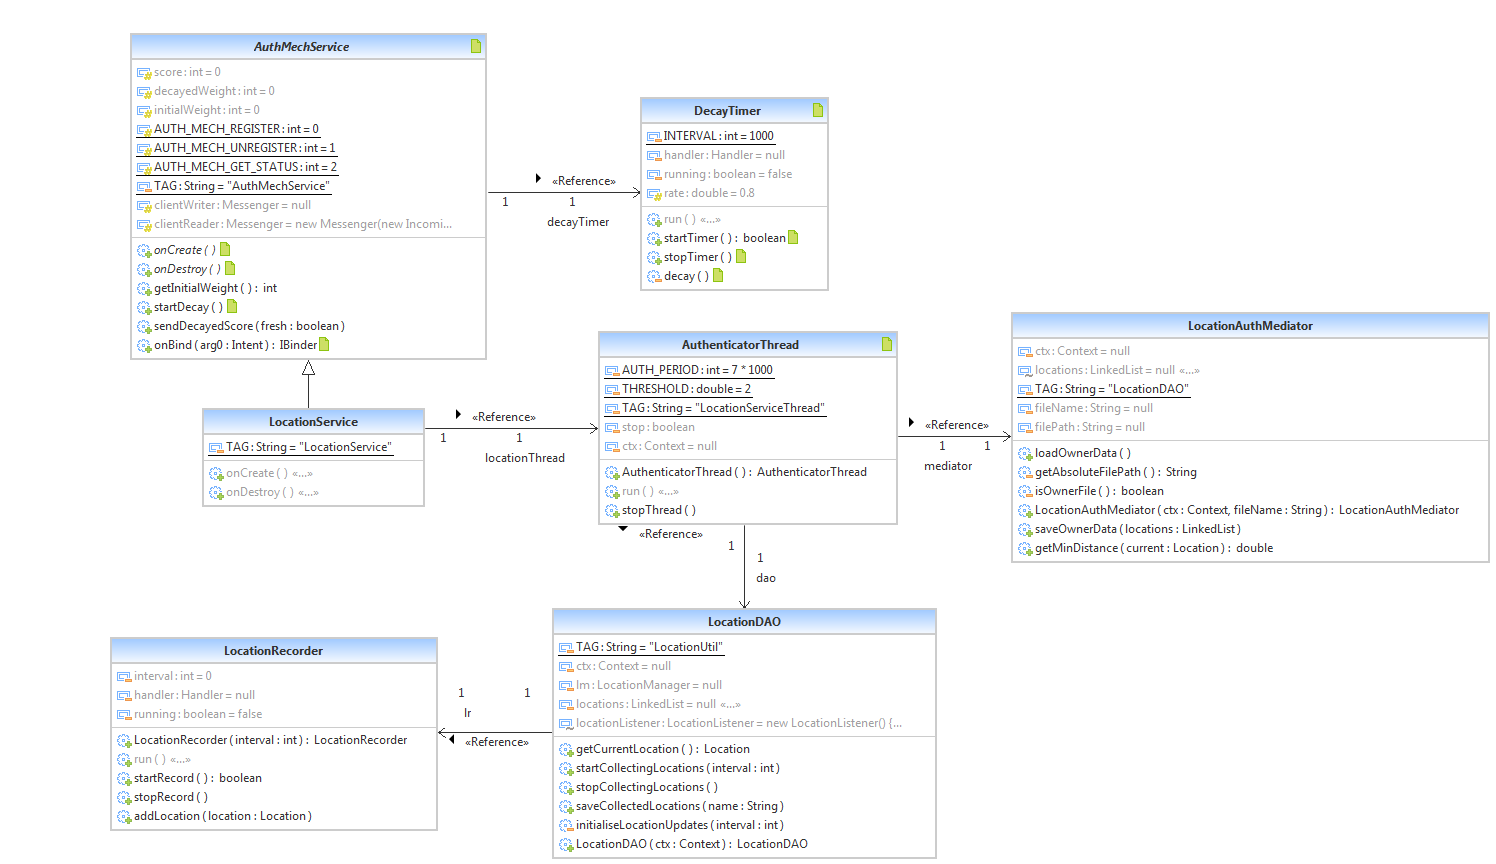
\includegraphics[width=\textwidth]{Pictures/location}
    \caption{Location analysis overview.}
    \label{fig:location}
\end{figure}

% DAO object used for collecting data
A DAO object is used to mediate Android API calls and manage the existing owner configuration. It is implemented in the ``LocationDAO'' class. It offers functionality for gathering and saving location updates. It is developed to use the most accurate data provider. The Android API offers the following sources of collecting ``Location'' data:
\begin{itemize}
	\item GPS\_PROVIDER: Collects data from the GPS.
	\item NETWORK\_PROVIDER: Collects data from cell tower and WiFi access points.
	\item PASSIVE\_PROVIDER: Passively collects data from other applications which receive ``Location'' updates.
\end{itemize}

% Describe the algorithm class
%	TODO: implement this with 5m
External libraries were not used for the authentication process. We have developed a primitive location analysis algorithm in the ``LocationAuthMediator'' class. During the configuration stage, which is a process managed by ``LocationActivity'', location data is sampled every 5 minutes and saved in internal storage. After the process has ended, each time a ``Location'' is sent for authentication it is compared with all the locations saved during the configuration process. The final result is the minimum number of meters between the current ``Location'' and any other saved ``Location''.

% Describe how authenticator thread works
When the ``LocationService'' mechanism is started, its ``onCreate()'' method spawns an authentication thread. This thread periodically requests the current location using the ``LocationDAO''. Data is returned in a ``Location'' object and is provided as input to the ``LocationAuthMediator''. Although the result is represented in meters, and is not an Euclidean distance, it can be converted to a percentage using equation \ref{eq:euclideantoprob}. Once the final probability is calculated, the weight decay process is restarted.

\subsection{Owner configuration}
% Owner configuration activities exist
There are a number of components that are used in the configuration of the prototype. Each authentication mechanism has a corresponding Activity that can be started from the main Activity called ``PicoUserAuthenticator''. These are used to register owner biometrics needed by the mechanisms.

% They use DAO objects to store data in internal storage
Each configuration Activity uses the same DAO class as its corresponding authentication mechanism. The DAO is used for collecting and storing owner data. Given that the overall size is relatively small, files are kept in internal storage.

\subsection{Cryptographic protection}
All biometric data registered by the owner and used by the mechanisms is stored in internal memory. This is protected by the Linux permissions model, and provides sufficient security from other applications. However, if an attacker acquires ``root'' privileges, the biometric files would be completely exposed. To add an additional layer of security, we have included cryptographic protection of owner data.

\begin{figure}[h]
    \centering
    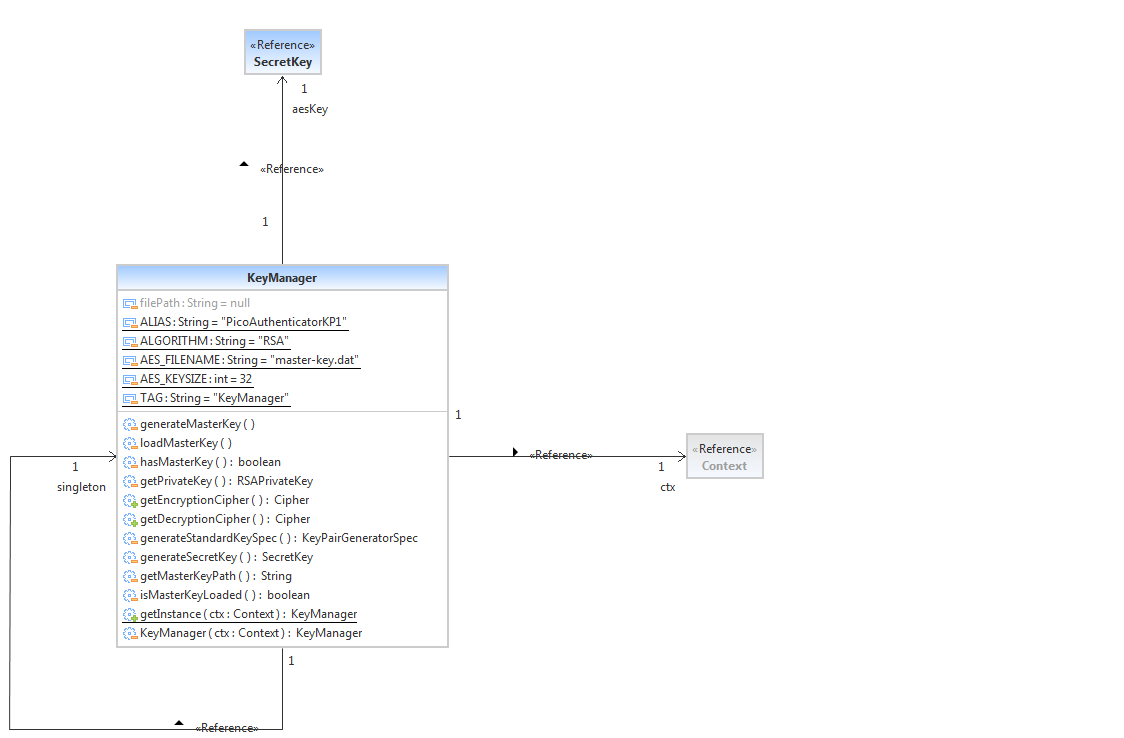
\includegraphics[width=0.7\textwidth]{Pictures/keymanager}
    \caption{KeyManager overview.}
    \label{fig:keymanager}
\end{figure}
The cryptographic layer is implemented in the ``KeyManager'' class. An overview of the class structure can be seen in figure \ref{fig:keymanager}. It uses the ``KeyStore'' API in order to keep an RSA key pair securely stored. Starting with Android 4.3, credentials stored in the Android ``KeyStore'' are not extractable because they are hardware secured using: Secure Element, TPM, or TrustZone. The securely stored RSA key pair is used to decrypt an AES master key that is kept encrypted in the app's internal memory. Once it is retrieved, the AES master key is used for encryption/decryption of configuration files.

All mechanisms except for face recognition use this cryptographic layer to keep data encrypted in internal memory. The face recognition mechanism does not support this feature due to the ``Javafaces'' library, which is implemented to process image files independently with no cryptographic support. 

\section{Conclusion}
% Small overall
We have described the Activity and Service components developed for the prototype, as well as their communication flow. We have ported two biometric libraries and developed a location analysis mechanism. DAO objects facilitate cryptographic access to owner configuration files, and additional classes mediate the calls to external libraries. An overview of the app design is available on github \footnote{https://github.com/cristiantoader/fyp-pico/blob/master/PicoUserAuthenticator/dissertation/Pictures/detailed-uml.png}.

% Limitations and solutions
One of the limitations of the prototype is the lack of explicit authentication mechanisms. Another issue is the precision of the biometric mechanisms, in the lack of better libraries. However, due to the modular design of the application, existing mechanisms can be improved simply by importing a new library and modifying the corresponding mediator class. The existing set of mechanisms can be increased by creating a new class that extends ``AuthMechService'' and implements the algorithm's logic. In order to be managed by ``UAService'', the new mechanism needs to be included in the ``UserAuthenticator.initAvailableDevices()'' method.

\section{Related work}
% Sensor sniffing
Liang Cai et al \cite{cai2009defending} analyse ways of protecting users from mobile phone sensor sniffing attacks. The authors design a framework used for protecting sensor data from being leaked. From a security perspective the user should not to be trusted with granting permissions to different applications. A solution provided in the paper is for sensors to become locked once they are used. A downside to this is that malware may deny service to legitimate applications by creating a race condition for acquiring a sensor lock. This can be solved by using an user notification, allowing for the owner to decide which application acquires the lock.

% Gait recognition
The paper by Derawi et al \cite{derawi2010unobtrusive} presents the feasibility of implementing gait authentication on Android as an unobtrusive unlocking mechanism. According to the definition offered by the authors ``gait recognition describes a biometric method which allows an automatic verification of the identity of a person by the way he walks''. The Android implementation developed by the authors has an equal error rate (EER) of $20\%$. Dedicated devices have an EER of only $12.9\%$, and the main cause for this is the sampling rate available at that time (2010). The authors have used a Google G1 phone with approximately 40-50 samples per second. This is much inferior to dedicated accelerometers that sample data at 100 samples per second. However, by conducting personal experiments with the accelerometer of a Google Nexus 5 phone, the rates of the highest sampling setting (SENSOR\_DELAY\_FASTEST) are over 100 samples per second. Therefore the current performance of the prototype developed in this paper should be closer to $12.9\%$.

% Improve speaker recognition in noisy conditions
Ming et al \cite{ming2007robust} present in their paper how to improve speaker recognition accuracy on mobile phone devices in noisy conditions. This approach uses a model training technique based on which missing features may be used to identify noise. The focus of the paper is designing and implementing the biometric mechanism.

% Voiceprints voice recognition
Another way of performing speaker recognition involves using voiceprints. These are a set of features extracted from the speaker sample data. Kersta \cite{kersta2005voiceprint} explains the mechanism in more detail. The benefit of having feature extraction, as opposed to a different voice recognition mechanism, is that voiceprints do not require any secrets. This increases the usability of the mechanism in different scenarios required by the Pico authenticator. However, a downside to this approach is that it makes replay attacks easier to perform. Any recording of the user is sufficient for an attacker to trick the biometric mechanism.

% Face recognition
A popular face recognition paper was written by Turk and Pentland \cite{turk1991face}. The biometric authentication process is based on the concept of ``eigenfaces''. This is a name given for the eigenvectors that are used to characterise the features of a face. These values are projected onto the feature space. Using Euclidean distances in the feature space, classification can be performed in order to identify users. An implementation of this mechanism was used with the Pico unlocking scheme prototype.

% Keystroke analysis
An unconventional authenticating mechanism is presented by Clarke and Furnell \cite{clarke2007authenticating}. They use keystroke analysis in order to make predictions regarding the user of a phone. This mechanism is unobtrusive and gathers data during normal user interactions such as typing a text message or phone number. It is based on a neural network classifier, reporting an EER of $12.8\%$. Input data used for classification is composed out of timings between successive keystrokes, and the hold time of a pressed key. 
